\begin{fullwidth}
\chapter{Circuit Quantum Electrodynamics}
\end{fullwidth}
\newthought{This chapter} is setup as notes to the transmon and to go through the theory leading to it. It is also training in writing in this format, so stuff might look a bit weird.  \\

\section{Circuit QED}
The basis is superconducting qubits is to use circuits to form our potential. By choosing to make the qubits of superconducting material, the energy dissipation is removed from the system and at low enough energies/temperatures this system will behave quantized as a quantum system. 

Classically\footnote{Following is from the Quantum engineers guide to Superconducting Qubits}, we define the dynamics of a circuit in terms of its current $I(t)$ and its voltage drop $V(t)$. Now to write up the Lagrangian in flux/charge basis which are conjugated variables. Using flux basis we define:
\begin{equation}
    \Phi (t) = \int_{-\infty}^t V(t')dt'
\end{equation}
Now using this relations together with $V = L dI/dt$ and $I = C dV/dt$ it is possible to find the energy by:
\marginnote[0.5 cm]{The lower integration limit comes from the assumption that the system was at rest at infinity}
\begin{equation}\label{eq: Energy from current and voltage}
    E(t) = \int_{-\infty}^t V(t')I(t')dt'
\end{equation}
Such that the energy of the components are:
\begin{equation}
    E_{capacitor} = \frac12 C \dot{\Phi}^2; \quad E_{inductor} = \frac{1}{2L} \Phi^2
\end{equation}
Defining the capacitant energy as the kinetic energy $T_C$ and inductive energy as $U_L$, we can write the Lagrangian as:
\begin{equation}
    \mathcal{L} = T_C - U_L = \frac12 C \dot{\Phi}^2 - \frac{1}{2L} \Phi^2
\end{equation}
And from this the Hamiltonian:\footnote{By defining a canonical momentum $Q = \partial \mathcal{L} / \partial \dot{\Phi}$ and doing the legendre transformation $\mathcal{H} = Q\dot{\Phi} - \mathcal{L}$.}:
\begin{equation}
    \mathcal{H} = \frac{1}{2C} Q^2 + \frac{1}{2L} \Phi^2
\end{equation}

\subsection{Going quantum}
$\Phi$ and $Q$ are classical, conjugate variables and satisfy the Poisson bracket:
\begin{equation}
    \{ \Phi, Q\} = \pfrac{\Phi}{\Phi}\pfrac{Q}{Q} - \pfrac{\Phi}{Q}\pfrac{Q}{\Phi} = 1
\end{equation}
To quantize these parameters, we replace the variables with the corresponding operators: $Q \to \hat{Q}$ and $\Phi \ \to \hat{\Phi}$. And using the correspondence principle to replace the Poisson brackets with the commutator $\{...\} \to i\hbar[...]$. We have \cite{krantz_quantum_2019}:
\begin{equation}
    [\hat{\Phi}, \hat{Q}] = i\hbar
\end{equation}



\section{Forming Qubits}
As a start, we consider the LC-circuit which consist of a single capacitive element and one inducting. This exactly yields the Hamiltonian $\mathcal{H} = \mathcal{H} = \frac{1}{2C} Q^2 + \frac{1}{2L} \Phi^2$. When considering a flux basis, we need 
\begin{marginfigure}[1 cm]
    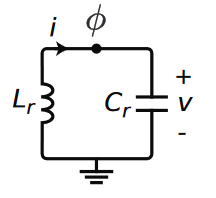
\includegraphics[width = \linewidth]{tex/fig_for_text/LC_circuit.png}
    \caption{Circuit diagram for the LC circuit.}
\end{marginfigure}
\begin{equation}
    \hat{Q} = i\hbar \pfrac{}{\hat{\Phi}}
\end{equation}
for the commutator relation to be satisfied. Dropping the hats and setting $\hbar = 1$
\begin{equation}
    H \ket{\psi} = - \frac{1}{2C} \pfracsquared{}{\Phi}\ket{\psi} + \frac{1}{2L} \Phi^2 \ket{\psi}
\end{equation}
Here we can follow the derivations from harmonic oscillators and define the ladder operators, $a, a^\dagger$. Such that the the Hamiltonian can be written as:
\begin{equation}
    H = \omega (a^\dagger a + \frac12)
\end{equation}
Where $\omega = \sqrt{8 E_C E_L}$ can be found by comparing the hamiltonian with the one from the harmonic oscillator.

While the harmonic oscillator has an abundance of nice properties for physics, it has equidistant energy levels. Driving oscillations with the frequency $\omega$ will not only contribute to transitions in the computational basis ($\ket{0}, \ket{1}$), but also all states $\ket{n}$ where $n > 1$. With this leakage quantum computing will be impossible, and for this reason, we must search for an anharmonic potential.

\subsection{The Josephson Junction}
The solution lies in another component, which is accessible in the superconducting circuit. By separating two superconductors by a semiconducting material, the Cooper pairs will no longer travel through without resistance but will instead have a probability of tunneling through the insulator/superconductor. This probability is dependent on the phase difference between the two superconductors. 
\marginnote[0.5 cm]{Probably an idea to derive the Josephson junction, maybe just for my own sake.}

The probability for tunneling through the superconducting phase is given as $\sin[2e\phi(t) / \hbar]$, where $\phi(t)$ is the time-dependent difference in phase between the two superconductors which are separated by the junction. Using the flux-quantum $\phi_0 = h / 2e$ and adding an external flux, the current through the Josephson Junction is:
\begin{equation}
    I(t) = I_0 \sin \left[ \frac{\phi(t) + \phi_{ext}}{\phi_0} \right]
\end{equation}
Which can be integrated according to equation \ref{eq: Energy from current and voltage} to get an energy:
\begin{equation}
    E_{\text{Josephson Junction}} = - E_J \cos \left[ \frac{\phi(t) + \phi_{ext}}{\phi_0} \right]
\end{equation}
up to a constant, which can be neglected by setting the zero point of the energy. \cite{vool_introduction_2017}

\subsection{The Cooper Pair Island}
Replacing the inductor with a Josephson Junction. We instead have a circuit with a non-quadratic energy term. We now have a Hamiltonian given by:

\begin{equation}
    H(t) =  4 E_C (n - n_g)^2 -  E_J \cos \left[ \frac{\phi(t) + \phi_{ext}}{\phi_0} \right]
\end{equation}

Which gives us an anharmonic potential.

\begin{marginfigure}
    \caption{An example of a circuit with a capacitor and a Josephson Junction}
    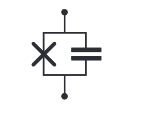
\includegraphics[width = \textwidth]{tex/fig_for_text/CooperPairIsland.png}
    \label{fig:cooper_pair_island}
\end{marginfigure}
\vspace{1 cm}
This section could also include the following:
\begin{itemize}
    \item A view of the potential and how the eigenstates lie in the potential.
    \item A comparison of the harmonic states with the states of the CPB. \\
    This would further motivate, that we define the anharmonicity and tell why it is effective. Drive a pulse with a narrow energy band must be long in time because of the fourier transform. \\
    \item In this narrative we can drive transitions between our computational subspace by using the mixing of our states in an avoided crossing. However, the energy states are here sensitive to the noise of our charge / applied voltage. 
\end{itemize}

\subsection{Drive Lines?}



\section{The Transmon}
The section must have the following:
\begin{itemize}
    \item How does the energy spectrum behave, when we increase the $E_J / E_C$ ratio. From 1 to 10 and to 50 where the Transmon lives.
    \begin{itemize}
        \item Compare the susceptibility to charge noise with the anhorminicty. We want to protect the qubit as well as possible while keeping the anharmonicity large, such that we can perform fast operations on the qubit. 
    \end{itemize}
\end{itemize}

\subsection{Solving the Transmon Numerically}
\textbf{This could also be a numerical section between section 2.1 and 2.2 which we can base the cooper pair box on. }
When using the transmon, we use the energy eigenstates as a computational basis. To figure out, how the energy splitting and reactions to charge are, we need to find these energy eigenenergies and states.

\begin{itemize}
    \item Start with charge basis
    \item We can now represent the flux as a potential
    \item Solving numerically gives lowest eigenenergy and states
    \item Calculating certain matrix elements between the eigenstates givers us the charge-matrix, flux-matrix, etc.. 
\end{itemize}


\section{Experimental Setup}
I should have this... Is this the right place? 

\subsection{Cooling}

\subsection{Amplication}

\subsection{Specs}








